\documentclass[twoside]{book}

% Packages required by doxygen
\usepackage{fixltx2e}
\usepackage{calc}
\usepackage{doxygen}
\usepackage[export]{adjustbox} % also loads graphicx
\usepackage{graphicx}
\usepackage[utf8]{inputenc}
\usepackage{makeidx}
\usepackage{multicol}
\usepackage{multirow}
\PassOptionsToPackage{warn}{textcomp}
\usepackage{textcomp}
\usepackage[nointegrals]{wasysym}
\usepackage[table]{xcolor}

% Font selection
\usepackage[T1]{fontenc}
\usepackage[scaled=.90]{helvet}
\usepackage{courier}
\usepackage{amssymb}
\usepackage{sectsty}
\renewcommand{\familydefault}{\sfdefault}
\allsectionsfont{%
  \fontseries{bc}\selectfont%
  \color{darkgray}%
}
\renewcommand{\DoxyLabelFont}{%
  \fontseries{bc}\selectfont%
  \color{darkgray}%
}
\newcommand{\+}{\discretionary{\mbox{\scriptsize$\hookleftarrow$}}{}{}}

% Page & text layout
\usepackage{geometry}
\geometry{%
  a4paper,%
  top=2.5cm,%
  bottom=2.5cm,%
  left=2.5cm,%
  right=2.5cm%
}
\tolerance=750
\hfuzz=15pt
\hbadness=750
\setlength{\emergencystretch}{15pt}
\setlength{\parindent}{0cm}
\setlength{\parskip}{3ex plus 2ex minus 2ex}
\makeatletter
\renewcommand{\paragraph}{%
  \@startsection{paragraph}{4}{0ex}{-1.0ex}{1.0ex}{%
    \normalfont\normalsize\bfseries\SS@parafont%
  }%
}
\renewcommand{\subparagraph}{%
  \@startsection{subparagraph}{5}{0ex}{-1.0ex}{1.0ex}{%
    \normalfont\normalsize\bfseries\SS@subparafont%
  }%
}
\makeatother

% Headers & footers
\usepackage{fancyhdr}
\pagestyle{fancyplain}
\fancyhead[LE]{\fancyplain{}{\bfseries\thepage}}
\fancyhead[CE]{\fancyplain{}{}}
\fancyhead[RE]{\fancyplain{}{\bfseries\leftmark}}
\fancyhead[LO]{\fancyplain{}{\bfseries\rightmark}}
\fancyhead[CO]{\fancyplain{}{}}
\fancyhead[RO]{\fancyplain{}{\bfseries\thepage}}
\fancyfoot[LE]{\fancyplain{}{}}
\fancyfoot[CE]{\fancyplain{}{}}
\fancyfoot[RE]{\fancyplain{}{\bfseries\scriptsize Generated by Doxygen }}
\fancyfoot[LO]{\fancyplain{}{\bfseries\scriptsize Generated by Doxygen }}
\fancyfoot[CO]{\fancyplain{}{}}
\fancyfoot[RO]{\fancyplain{}{}}
\renewcommand{\footrulewidth}{0.4pt}
\renewcommand{\chaptermark}[1]{%
  \markboth{#1}{}%
}
\renewcommand{\sectionmark}[1]{%
  \markright{\thesection\ #1}%
}

% Indices & bibliography
\usepackage{natbib}
\usepackage[titles]{tocloft}
\setcounter{tocdepth}{3}
\setcounter{secnumdepth}{5}
\makeindex

% Hyperlinks (required, but should be loaded last)
\usepackage{ifpdf}
\ifpdf
  \usepackage[pdftex,pagebackref=true]{hyperref}
\else
  \usepackage[ps2pdf,pagebackref=true]{hyperref}
\fi
\hypersetup{%
  colorlinks=true,%
  linkcolor=blue,%
  citecolor=blue,%
  unicode%
}

% Custom commands
\newcommand{\clearemptydoublepage}{%
  \newpage{\pagestyle{empty}\cleardoublepage}%
}

\usepackage{caption}
\captionsetup{labelsep=space,justification=centering,font={bf},singlelinecheck=off,skip=4pt,position=top}

%===== C O N T E N T S =====

\begin{document}

% Titlepage & ToC
\hypersetup{pageanchor=false,
             bookmarksnumbered=true,
             pdfencoding=unicode
            }
\pagenumbering{roman}
\begin{titlepage}
\vspace*{7cm}
\begin{center}%
{\Large My Project }\\
\vspace*{1cm}
{\large Generated by Doxygen 1.8.11}\\
\end{center}
\end{titlepage}
\clearemptydoublepage
\tableofcontents
\clearemptydoublepage
\pagenumbering{arabic}
\hypersetup{pageanchor=true}

%--- Begin generated contents ---
\chapter{Class Index}
\section{Class List}
Here are the classes, structs, unions and interfaces with brief descriptions\+:\begin{DoxyCompactList}
\item\contentsline{section}{\hyperlink{classmongoapi_1_1MongoInterface}{mongoapi\+::\+Mongo\+Interface} \\*An interface to a Mongo\+DB database with methods to insert, retrieve, and remove entries with Json\+Box Values }{\pageref{classmongoapi_1_1MongoInterface}}{}
\end{DoxyCompactList}

\chapter{File Index}
\section{File List}
Here is a list of all documented files with brief descriptions\+:\begin{DoxyCompactList}
\item\contentsline{section}{\hyperlink{mongoapi_8h}{mongoapi.\+h} }{\pageref{mongoapi_8h}}{}
\end{DoxyCompactList}

\chapter{Class Documentation}
\hypertarget{classmongoapi_1_1MongoInterface}{}\section{mongoapi\+:\+:Mongo\+Interface Class Reference}
\label{classmongoapi_1_1MongoInterface}\index{mongoapi\+::\+Mongo\+Interface@{mongoapi\+::\+Mongo\+Interface}}


An interface to a Mongo\+DB database with methods to insert, retrieve, and remove entries with Json\+Box Values.  




{\ttfamily \#include $<$mongoapi.\+h$>$}

\subsection*{Public Member Functions}
\begin{DoxyCompactItemize}
\item 
\hyperlink{classmongoapi_1_1MongoInterface_ab0be108c960a6cb1cf926e90c67dc6a2}{Mongo\+Interface} (std\+::string database, std\+::string U\+RI=\char`\"{}127.\+0.\+0.\+1\+:27017\char`\"{})
\item 
virtual \hyperlink{classmongoapi_1_1MongoInterface_ab04b30920b692570cf39a232bad39e31}{$\sim$\+Mongo\+Interface} ()
\item 
bool \hyperlink{classmongoapi_1_1MongoInterface_abd351b10712380d3cc3a9fdfea045816}{insert\+J\+S\+ON} (std\+::string collection, Json\+Box\+::\+Value data)
\item 
Json\+Box\+::\+Value \hyperlink{classmongoapi_1_1MongoInterface_a5be1cd9378f89523963212a58c126205}{query} (std\+::string collection, Json\+Box\+::\+Value data)
\item 
Json\+Box\+::\+Value \hyperlink{classmongoapi_1_1MongoInterface_ae85cc136f15074ba9e7dabcc7de1ac0b}{query\+All} (std\+::string collection)
\item 
bool \hyperlink{classmongoapi_1_1MongoInterface_a3ef36851d7f551223f72faa6bb355f99}{remove\+Entry} (std\+::string collection, Json\+Box\+::\+Value data)
\item 
bool \hyperlink{classmongoapi_1_1MongoInterface_a2dccbb59fb1fd7ea81d946e84e592561}{update} (std\+::string collection, Json\+Box\+::\+Value filter, Json\+Box\+::\+Value update)
\item 
int \hyperlink{classmongoapi_1_1MongoInterface_ad938ece65fafa37c0517f20fcf0fed9d}{count} (std\+::string collection)
\item 
int \hyperlink{classmongoapi_1_1MongoInterface_a889dc36348bbb47d0867c628d3c8534e}{count\+Filter} (std\+::string collection, Json\+Box\+::\+Value filter)
\item 
std\+::string \hyperlink{classmongoapi_1_1MongoInterface_a39d9fd2dc8b9bf2e6b9590504d02a811}{get\+Database} () const 
\item 
std\+::string \hyperlink{classmongoapi_1_1MongoInterface_a7f95673d3c950679fb64190862c127fc}{get\+U\+RI} () const 
\item 
bool \hyperlink{classmongoapi_1_1MongoInterface_a3721592cc497178f8c8e0567c7439991}{remove\+All\+Entries} (std\+::string collection)
\item 
bool \hyperlink{classmongoapi_1_1MongoInterface_a18c2763a4f06cf1e717875007bb47963}{drop\+Collection} (std\+::string collection)
\end{DoxyCompactItemize}


\subsection{Detailed Description}
An interface to a Mongo\+DB database with methods to insert, retrieve, and remove entries with Json\+Box Values. 

\subsection{Constructor \& Destructor Documentation}
\index{mongoapi\+::\+Mongo\+Interface@{mongoapi\+::\+Mongo\+Interface}!Mongo\+Interface@{Mongo\+Interface}}
\index{Mongo\+Interface@{Mongo\+Interface}!mongoapi\+::\+Mongo\+Interface@{mongoapi\+::\+Mongo\+Interface}}
\subsubsection[{\texorpdfstring{Mongo\+Interface(std\+::string database, std\+::string U\+R\+I=""127.\+0.\+0.\+1\+:27017"")}{MongoInterface(std::string database, std::string URI="127.0.0.1:27017")}}]{\setlength{\rightskip}{0pt plus 5cm}mongoapi\+::\+Mongo\+Interface\+::\+Mongo\+Interface (
\begin{DoxyParamCaption}
\item[{std\+::string}]{database, }
\item[{std\+::string}]{U\+RI = {\ttfamily \char`\"{}127.0.0.1\+:27017\char`\"{}}}
\end{DoxyParamCaption}
)}\hypertarget{classmongoapi_1_1MongoInterface_ab0be108c960a6cb1cf926e90c67dc6a2}{}\label{classmongoapi_1_1MongoInterface_ab0be108c960a6cb1cf926e90c67dc6a2}
Constructor opens connection to database with specified name.


\begin{DoxyParams}{Parameters}
{\em database} & Name of the database to connect to \\
\hline
{\em U\+RI} & The IP address and port given as a string in the form \char`\"{}\+I\+P\+:\+Port\char`\"{} default\+: \char`\"{}127.\+0.\+0.\+1\+:27017\char`\"{} \\
\hline
\end{DoxyParams}
\index{mongoapi\+::\+Mongo\+Interface@{mongoapi\+::\+Mongo\+Interface}!````~Mongo\+Interface@{$\sim$\+Mongo\+Interface}}
\index{````~Mongo\+Interface@{$\sim$\+Mongo\+Interface}!mongoapi\+::\+Mongo\+Interface@{mongoapi\+::\+Mongo\+Interface}}
\subsubsection[{\texorpdfstring{$\sim$\+Mongo\+Interface()}{~MongoInterface()}}]{\setlength{\rightskip}{0pt plus 5cm}mongoapi\+::\+Mongo\+Interface\+::$\sim$\+Mongo\+Interface (
\begin{DoxyParamCaption}
{}
\end{DoxyParamCaption}
)\hspace{0.3cm}{\ttfamily [virtual]}}\hypertarget{classmongoapi_1_1MongoInterface_ab04b30920b692570cf39a232bad39e31}{}\label{classmongoapi_1_1MongoInterface_ab04b30920b692570cf39a232bad39e31}
Destructor 

\subsection{Member Function Documentation}
\index{mongoapi\+::\+Mongo\+Interface@{mongoapi\+::\+Mongo\+Interface}!count@{count}}
\index{count@{count}!mongoapi\+::\+Mongo\+Interface@{mongoapi\+::\+Mongo\+Interface}}
\subsubsection[{\texorpdfstring{count(std\+::string collection)}{count(std::string collection)}}]{\setlength{\rightskip}{0pt plus 5cm}int mongoapi\+::\+Mongo\+Interface\+::count (
\begin{DoxyParamCaption}
\item[{std\+::string}]{collection}
\end{DoxyParamCaption}
)}\hypertarget{classmongoapi_1_1MongoInterface_ad938ece65fafa37c0517f20fcf0fed9d}{}\label{classmongoapi_1_1MongoInterface_ad938ece65fafa37c0517f20fcf0fed9d}
Count the number of objects in the collection specified


\begin{DoxyParams}{Parameters}
{\em collection} & The name of the collection to query \\
\hline
\end{DoxyParams}
\begin{DoxyReturn}{Returns}
Integer value of number 
\end{DoxyReturn}
\index{mongoapi\+::\+Mongo\+Interface@{mongoapi\+::\+Mongo\+Interface}!count\+Filter@{count\+Filter}}
\index{count\+Filter@{count\+Filter}!mongoapi\+::\+Mongo\+Interface@{mongoapi\+::\+Mongo\+Interface}}
\subsubsection[{\texorpdfstring{count\+Filter(std\+::string collection, Json\+Box\+::\+Value filter)}{countFilter(std::string collection, JsonBox::Value filter)}}]{\setlength{\rightskip}{0pt plus 5cm}int mongoapi\+::\+Mongo\+Interface\+::count\+Filter (
\begin{DoxyParamCaption}
\item[{std\+::string}]{collection, }
\item[{Json\+Box\+::\+Value}]{filter}
\end{DoxyParamCaption}
)}\hypertarget{classmongoapi_1_1MongoInterface_a889dc36348bbb47d0867c628d3c8534e}{}\label{classmongoapi_1_1MongoInterface_a889dc36348bbb47d0867c628d3c8534e}
Count the number of objects in the collection specified that match the specified filter


\begin{DoxyParams}{Parameters}
{\em collection} & The name of the collection to query \\
\hline
{\em filter} & The query used on collection \\
\hline
\end{DoxyParams}
\begin{DoxyReturn}{Returns}
Integer value of number 
\end{DoxyReturn}
\index{mongoapi\+::\+Mongo\+Interface@{mongoapi\+::\+Mongo\+Interface}!drop\+Collection@{drop\+Collection}}
\index{drop\+Collection@{drop\+Collection}!mongoapi\+::\+Mongo\+Interface@{mongoapi\+::\+Mongo\+Interface}}
\subsubsection[{\texorpdfstring{drop\+Collection(std\+::string collection)}{dropCollection(std::string collection)}}]{\setlength{\rightskip}{0pt plus 5cm}bool mongoapi\+::\+Mongo\+Interface\+::drop\+Collection (
\begin{DoxyParamCaption}
\item[{std\+::string}]{collection}
\end{DoxyParamCaption}
)}\hypertarget{classmongoapi_1_1MongoInterface_a18c2763a4f06cf1e717875007bb47963}{}\label{classmongoapi_1_1MongoInterface_a18c2763a4f06cf1e717875007bb47963}
Drop specified collection


\begin{DoxyParams}{Parameters}
{\em collection} & The name of the collection \\
\hline
\end{DoxyParams}
\begin{DoxyReturn}{Returns}
True on success 
\end{DoxyReturn}
\index{mongoapi\+::\+Mongo\+Interface@{mongoapi\+::\+Mongo\+Interface}!get\+Database@{get\+Database}}
\index{get\+Database@{get\+Database}!mongoapi\+::\+Mongo\+Interface@{mongoapi\+::\+Mongo\+Interface}}
\subsubsection[{\texorpdfstring{get\+Database() const }{getDatabase() const }}]{\setlength{\rightskip}{0pt plus 5cm}std\+::string mongoapi\+::\+Mongo\+Interface\+::get\+Database (
\begin{DoxyParamCaption}
{}
\end{DoxyParamCaption}
) const}\hypertarget{classmongoapi_1_1MongoInterface_a39d9fd2dc8b9bf2e6b9590504d02a811}{}\label{classmongoapi_1_1MongoInterface_a39d9fd2dc8b9bf2e6b9590504d02a811}
Returns a string containing the name of the current database

\begin{DoxyReturn}{Returns}
The name of the current database 
\end{DoxyReturn}
\index{mongoapi\+::\+Mongo\+Interface@{mongoapi\+::\+Mongo\+Interface}!get\+U\+RI@{get\+U\+RI}}
\index{get\+U\+RI@{get\+U\+RI}!mongoapi\+::\+Mongo\+Interface@{mongoapi\+::\+Mongo\+Interface}}
\subsubsection[{\texorpdfstring{get\+U\+R\+I() const }{getURI() const }}]{\setlength{\rightskip}{0pt plus 5cm}std\+::string mongoapi\+::\+Mongo\+Interface\+::get\+U\+RI (
\begin{DoxyParamCaption}
{}
\end{DoxyParamCaption}
) const}\hypertarget{classmongoapi_1_1MongoInterface_a7f95673d3c950679fb64190862c127fc}{}\label{classmongoapi_1_1MongoInterface_a7f95673d3c950679fb64190862c127fc}
Returns a string containing the IP and Port of the database

\begin{DoxyReturn}{Returns}
The IP and port in the form \char`\"{}\+I\+P\+:\+Port\char`\"{} 
\end{DoxyReturn}
\index{mongoapi\+::\+Mongo\+Interface@{mongoapi\+::\+Mongo\+Interface}!insert\+J\+S\+ON@{insert\+J\+S\+ON}}
\index{insert\+J\+S\+ON@{insert\+J\+S\+ON}!mongoapi\+::\+Mongo\+Interface@{mongoapi\+::\+Mongo\+Interface}}
\subsubsection[{\texorpdfstring{insert\+J\+S\+O\+N(std\+::string collection, Json\+Box\+::\+Value data)}{insertJSON(std::string collection, JsonBox::Value data)}}]{\setlength{\rightskip}{0pt plus 5cm}bool mongoapi\+::\+Mongo\+Interface\+::insert\+J\+S\+ON (
\begin{DoxyParamCaption}
\item[{std\+::string}]{collection, }
\item[{Json\+Box\+::\+Value}]{data}
\end{DoxyParamCaption}
)}\hypertarget{classmongoapi_1_1MongoInterface_abd351b10712380d3cc3a9fdfea045816}{}\label{classmongoapi_1_1MongoInterface_abd351b10712380d3cc3a9fdfea045816}
Insert a Json\+Box Value into the database with specified collection.


\begin{DoxyParams}{Parameters}
{\em collection} & The name of the collection to insert Value into \\
\hline
{\em data} & The Json\+Box Value to insert \\
\hline
\end{DoxyParams}
\begin{DoxyReturn}{Returns}
True on success 
\end{DoxyReturn}
\index{mongoapi\+::\+Mongo\+Interface@{mongoapi\+::\+Mongo\+Interface}!query@{query}}
\index{query@{query}!mongoapi\+::\+Mongo\+Interface@{mongoapi\+::\+Mongo\+Interface}}
\subsubsection[{\texorpdfstring{query(std\+::string collection, Json\+Box\+::\+Value data)}{query(std::string collection, JsonBox::Value data)}}]{\setlength{\rightskip}{0pt plus 5cm}Json\+Box\+::\+Value mongoapi\+::\+Mongo\+Interface\+::query (
\begin{DoxyParamCaption}
\item[{std\+::string}]{collection, }
\item[{Json\+Box\+::\+Value}]{data}
\end{DoxyParamCaption}
)}\hypertarget{classmongoapi_1_1MongoInterface_a5be1cd9378f89523963212a58c126205}{}\label{classmongoapi_1_1MongoInterface_a5be1cd9378f89523963212a58c126205}
Query the specified collection according to a specified Json\+Box Value


\begin{DoxyParams}{Parameters}
{\em collection} & The name of the collection to query \\
\hline
{\em data} & The Json\+Box Value query \\
\hline
\end{DoxyParams}
\begin{DoxyReturn}{Returns}
Array of results 
\end{DoxyReturn}
\index{mongoapi\+::\+Mongo\+Interface@{mongoapi\+::\+Mongo\+Interface}!query\+All@{query\+All}}
\index{query\+All@{query\+All}!mongoapi\+::\+Mongo\+Interface@{mongoapi\+::\+Mongo\+Interface}}
\subsubsection[{\texorpdfstring{query\+All(std\+::string collection)}{queryAll(std::string collection)}}]{\setlength{\rightskip}{0pt plus 5cm}Json\+Box\+::\+Value mongoapi\+::\+Mongo\+Interface\+::query\+All (
\begin{DoxyParamCaption}
\item[{std\+::string}]{collection}
\end{DoxyParamCaption}
)}\hypertarget{classmongoapi_1_1MongoInterface_ae85cc136f15074ba9e7dabcc7de1ac0b}{}\label{classmongoapi_1_1MongoInterface_ae85cc136f15074ba9e7dabcc7de1ac0b}
Query the specified collection for all Json\+Box Values


\begin{DoxyParams}{Parameters}
{\em collection} & The name of the collection to query \\
\hline
\end{DoxyParams}
\begin{DoxyReturn}{Returns}
Array of results 
\end{DoxyReturn}
\index{mongoapi\+::\+Mongo\+Interface@{mongoapi\+::\+Mongo\+Interface}!remove\+All\+Entries@{remove\+All\+Entries}}
\index{remove\+All\+Entries@{remove\+All\+Entries}!mongoapi\+::\+Mongo\+Interface@{mongoapi\+::\+Mongo\+Interface}}
\subsubsection[{\texorpdfstring{remove\+All\+Entries(std\+::string collection)}{removeAllEntries(std::string collection)}}]{\setlength{\rightskip}{0pt plus 5cm}bool mongoapi\+::\+Mongo\+Interface\+::remove\+All\+Entries (
\begin{DoxyParamCaption}
\item[{std\+::string}]{collection}
\end{DoxyParamCaption}
)}\hypertarget{classmongoapi_1_1MongoInterface_a3721592cc497178f8c8e0567c7439991}{}\label{classmongoapi_1_1MongoInterface_a3721592cc497178f8c8e0567c7439991}
Remove all entries from the specified collection


\begin{DoxyParams}{Parameters}
{\em collection} & The name of the collection \\
\hline
\end{DoxyParams}
\begin{DoxyReturn}{Returns}
True on success 
\end{DoxyReturn}
\index{mongoapi\+::\+Mongo\+Interface@{mongoapi\+::\+Mongo\+Interface}!remove\+Entry@{remove\+Entry}}
\index{remove\+Entry@{remove\+Entry}!mongoapi\+::\+Mongo\+Interface@{mongoapi\+::\+Mongo\+Interface}}
\subsubsection[{\texorpdfstring{remove\+Entry(std\+::string collection, Json\+Box\+::\+Value data)}{removeEntry(std::string collection, JsonBox::Value data)}}]{\setlength{\rightskip}{0pt plus 5cm}bool mongoapi\+::\+Mongo\+Interface\+::remove\+Entry (
\begin{DoxyParamCaption}
\item[{std\+::string}]{collection, }
\item[{Json\+Box\+::\+Value}]{data}
\end{DoxyParamCaption}
)}\hypertarget{classmongoapi_1_1MongoInterface_a3ef36851d7f551223f72faa6bb355f99}{}\label{classmongoapi_1_1MongoInterface_a3ef36851d7f551223f72faa6bb355f99}
Remove one or multiple entries from the specified collection


\begin{DoxyParams}{Parameters}
{\em collection} & The name of the collection \\
\hline
{\em data} & A Json\+Box Value specifying what entries to remove \\
\hline
\end{DoxyParams}
\begin{DoxyReturn}{Returns}
True on success 
\end{DoxyReturn}
\index{mongoapi\+::\+Mongo\+Interface@{mongoapi\+::\+Mongo\+Interface}!update@{update}}
\index{update@{update}!mongoapi\+::\+Mongo\+Interface@{mongoapi\+::\+Mongo\+Interface}}
\subsubsection[{\texorpdfstring{update(std\+::string collection, Json\+Box\+::\+Value filter, Json\+Box\+::\+Value update)}{update(std::string collection, JsonBox::Value filter, JsonBox::Value update)}}]{\setlength{\rightskip}{0pt plus 5cm}bool mongoapi\+::\+Mongo\+Interface\+::update (
\begin{DoxyParamCaption}
\item[{std\+::string}]{collection, }
\item[{Json\+Box\+::\+Value}]{filter, }
\item[{Json\+Box\+::\+Value}]{update}
\end{DoxyParamCaption}
)}\hypertarget{classmongoapi_1_1MongoInterface_a2dccbb59fb1fd7ea81d946e84e592561}{}\label{classmongoapi_1_1MongoInterface_a2dccbb59fb1fd7ea81d946e84e592561}
this queries a collection for the specified value, and updates it with the passed parameters. This function will only update one entry if the query matches multiple.


\begin{DoxyParams}{Parameters}
{\em collection} & The name of the collection \\
\hline
{\em filter} & Which entry to update \\
\hline
{\em update} & The parameters to update with \\
\hline
\end{DoxyParams}
\begin{DoxyReturn}{Returns}
True on success 
\end{DoxyReturn}


The documentation for this class was generated from the following files\+:\begin{DoxyCompactItemize}
\item 
\hyperlink{mongoapi_8h}{mongoapi.\+h}\item 
mongoapi.\+cpp\end{DoxyCompactItemize}

\chapter{File Documentation}
\hypertarget{mongoapi_8h}{}\section{mongoapi.\+h File Reference}
\label{mongoapi_8h}\index{mongoapi.\+h@{mongoapi.\+h}}
{\ttfamily \#include $<$cstdlib$>$}\\*
{\ttfamily \#include $<$iostream$>$}\\*
{\ttfamily \#include $<$sstream$>$}\\*
{\ttfamily \#include $<$fstream$>$}\\*
{\ttfamily \#include \char`\"{}Json\+Box.\+h\char`\"{}}\\*
{\ttfamily \#include $<$vector$>$}\\*
{\ttfamily \#include $<$bsoncxx/json.\+hpp$>$}\\*
{\ttfamily \#include $<$mongocxx/client.\+hpp$>$}\\*
{\ttfamily \#include $<$mongocxx/instance.\+hpp$>$}\\*
{\ttfamily \#include $<$mongocxx/stdx.\+hpp$>$}\\*
{\ttfamily \#include $<$mongocxx/uri.\+hpp$>$}\\*
{\ttfamily \#include $<$mongocxx/exception/bulk\+\_\+write\+\_\+exception.\+hpp$>$}\\*
{\ttfamily \#include $<$assert.\+h$>$}\\*
{\ttfamily \#include $<$aquetitools/\+Timer.\+h$>$}\\*
{\ttfamily \#include $<$mongoapi/revision.\+h$>$}\\*
{\ttfamily \#include $<$aquetitools/revision.\+h$>$}\\*
Include dependency graph for mongoapi.\+h\+:
\nopagebreak
\begin{figure}[H]
\begin{center}
\leavevmode
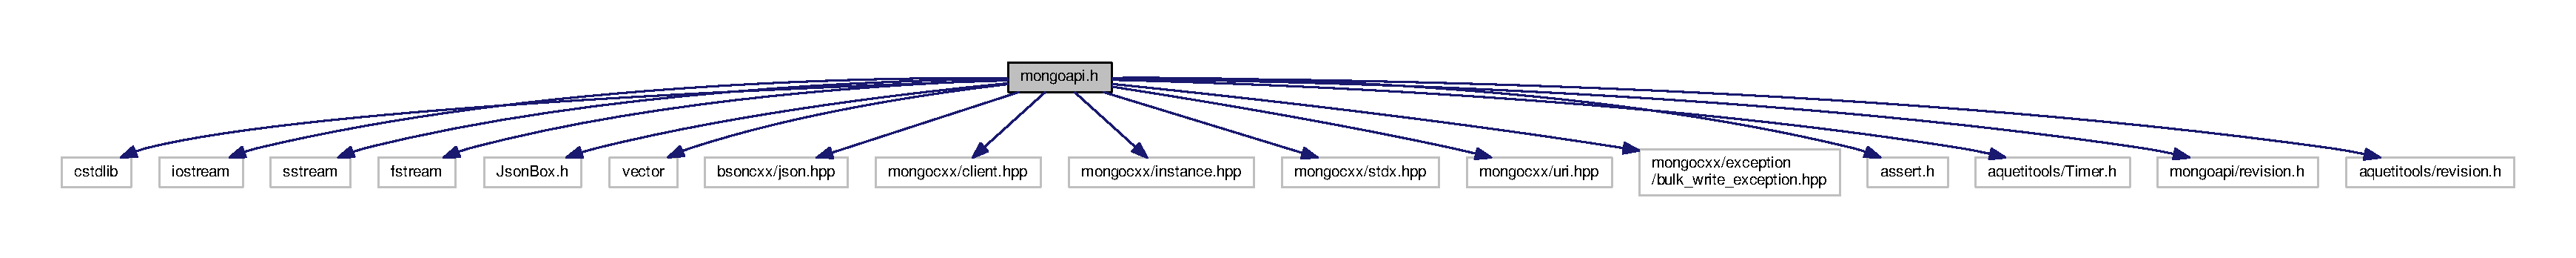
\includegraphics[width=350pt]{mongoapi_8h__incl}
\end{center}
\end{figure}
\subsection*{Classes}
\begin{DoxyCompactItemize}
\item 
class \hyperlink{classmongoapi_1_1MongoInterface}{mongoapi\+::\+Mongo\+Interface}
\begin{DoxyCompactList}\small\item\em An interface to a Mongo\+DB database with methods to insert, retrieve, and remove entries with Json\+Box Values. \end{DoxyCompactList}\end{DoxyCompactItemize}
\subsection*{Functions}
\begin{DoxyCompactItemize}
\item 
std\+::string {\bfseries mongoapi\+::test\+Mongo\+Interface} (bool print\+Flag, bool asser\+Flag)
\end{DoxyCompactItemize}


\subsection{Detailed Description}
\begin{DoxyAuthor}{Author}
Nils Persson \href{mailto:npersson@live.unc.edu}{\tt npersson@live.\+unc.\+edu} 
\end{DoxyAuthor}
\begin{DoxyVersion}{Version}
1.\+0
\end{DoxyVersion}
Interface class to Mongo\+DB

A class to connect to a Mongo\+DB database with methods to insert, retrieve, and remove entries with Json\+Box Values. 

\subsection{Function Documentation}
\index{mongoapi.\+h@{mongoapi.\+h}!test\+Mongo\+Interface@{test\+Mongo\+Interface}}
\index{test\+Mongo\+Interface@{test\+Mongo\+Interface}!mongoapi.\+h@{mongoapi.\+h}}
\subsubsection[{\texorpdfstring{test\+Mongo\+Interface(bool print\+Flag, bool asser\+Flag)}{testMongoInterface(bool printFlag, bool asserFlag)}}]{\setlength{\rightskip}{0pt plus 5cm}std\+::string mongoapi\+::test\+Mongo\+Interface (
\begin{DoxyParamCaption}
\item[{bool}]{print\+Flag, }
\item[{bool}]{assert\+Flag}
\end{DoxyParamCaption}
)}\hypertarget{mongoapi_8cpp_file_a6578d7b7ffba7800730cbbcb295ad528}{}\label{mongoapi_8cpp_file_a6578d7b7ffba7800730cbbcb295ad528}
Perform unit tests for the mongoapi class


\begin{DoxyParams}{Parameters}
{\em print\+Flag} & The boolean, true if printed messages to console desired \\
\hline
{\em assert\+Flag} & The boolean, true if quit desired upon error \\
\hline
\end{DoxyParams}
\begin{DoxyReturn}{Returns}
True on success 
\end{DoxyReturn}

%--- End generated contents ---

% Index
\backmatter
\newpage
\phantomsection
\clearemptydoublepage
\addcontentsline{toc}{chapter}{Index}
\printindex

\end{document}
